
% Diapositiva 1: Introducción a MediaPipe
\begin{frame}{¿Qué es MediaPipe?}
    \begin{itemize}
        \item Es una biblioteca de código abierto de Google para procesamiento de señales en tiempo real.
        \item Permite la implementación de modelos de Machine Learning en dispositivos móviles y de escritorio.
        \item Soporta múltiples plataformas como Android, iOS, y Python.
    \end{itemize}
    Flujo de Procesamiento:
    \begin{enumerate}
        \item Captura de datos desde una cámara o archivo.
        \item Procesamiento mediante el gráfico de MediaPipe.
        \item Obtención de resultados como coordenadas de puntos clave o segmentación.
    \end{enumerate}

\end{frame}

% Diapositiva 3: Soluciones preentrenadas
\begin{frame}{Soluciones preentrenadas}
    \textbf{Detección facial:} Seguimiento de rasgos faciales para aplicaciones como realidad aumentada y reconocimiento facial.
     \begin{itemize}
        \item Utiliza una malla 3D con 468 puntos clave en el rostro.
        \item Permite el reconocimiento detallado de expresiones faciales y contornos.
        \item Funciona en tiempo real para aplicaciones como filtros de realidad aumentada y seguimiento facial.
        \item Proporciona una representación tridimensional sin necesidad de sensores de profundidad.
    \end{itemize}
    \begin{center}
        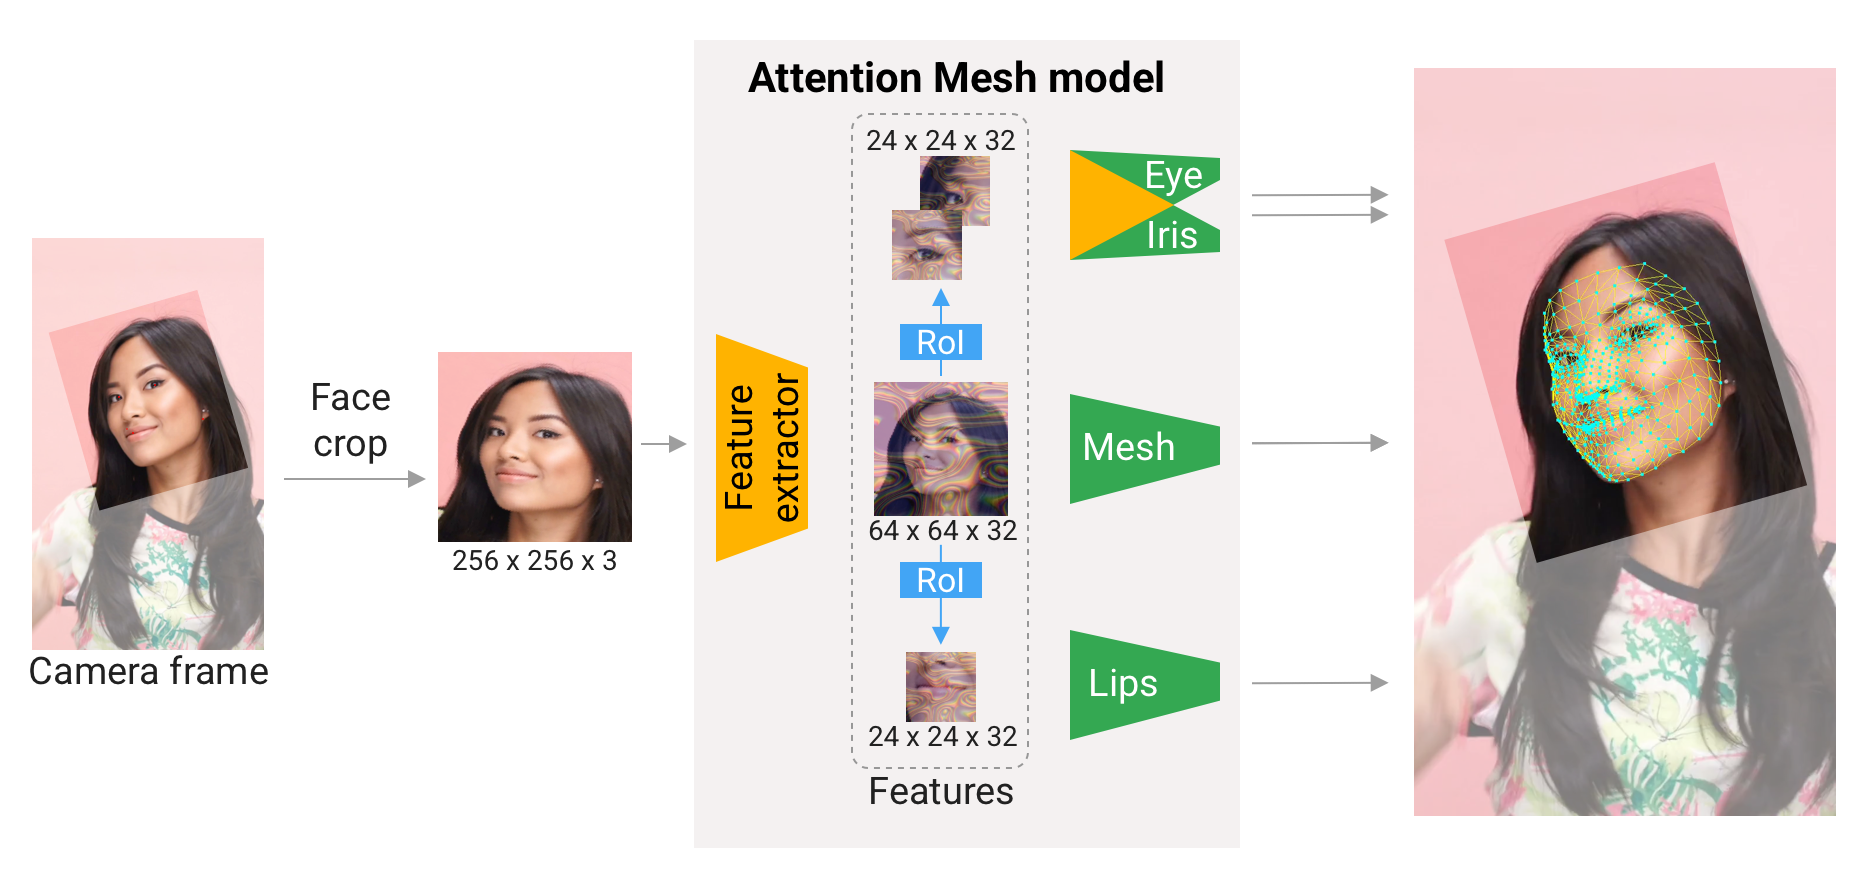
\includegraphics[width=0.6\linewidth]{01_MediaPipe/fase_mesh_detection.png}
    \end{center}
\end{frame}

\begin{frame}{Soluciones preentrenadas}
    \textbf{Detección de pose:} Identificación de puntos clave en el cuerpo humano para análisis de movimiento.
    \begin{itemize}
        \item Utiliza modelos de aprendizaje profundo para identificar 33 puntos clave en el cuerpo humano.
        \item Procesa imágenes en tiempo real desde la cámara o archivos de video.
        \item Genera un esqueleto virtual basado en las coordenadas de los puntos detectados.
        \item Se emplea en aplicaciones como deportes, rehabilitación y realidad aumentada.
    \end{itemize}    
    \begin{center}
        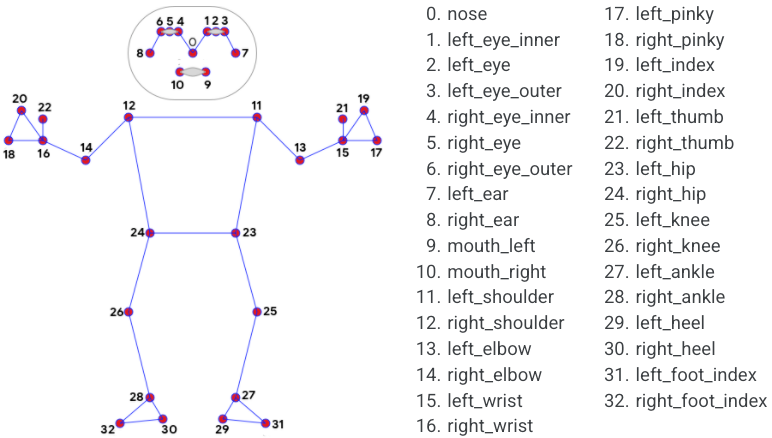
\includegraphics[width=0.6\linewidth]{01_MediaPipe/pose_landmarks.png}
    \end{center}
\end{frame}

\begin{frame}{Soluciones preentrenadas}
   \textbf{Detección de manos:} Segmentación y seguimiento de manos en tiempo real para gestos y control por movimientos.
   \begin{itemize}
        \item Detecta 21 puntos clave en cada mano utilizando modelos de Machine Learning.
        \item Funciona en tiempo real, permitiendo el seguimiento preciso de los movimientos de la mano.
        \item Se utiliza en aplicaciones como control por gestos, realidad aumentada y comunicación en lenguaje de señas.
        \item Proporciona coordenadas tridimensionales sin necesidad de sensores adicionales.
    \end{itemize}
    \begin{center}
        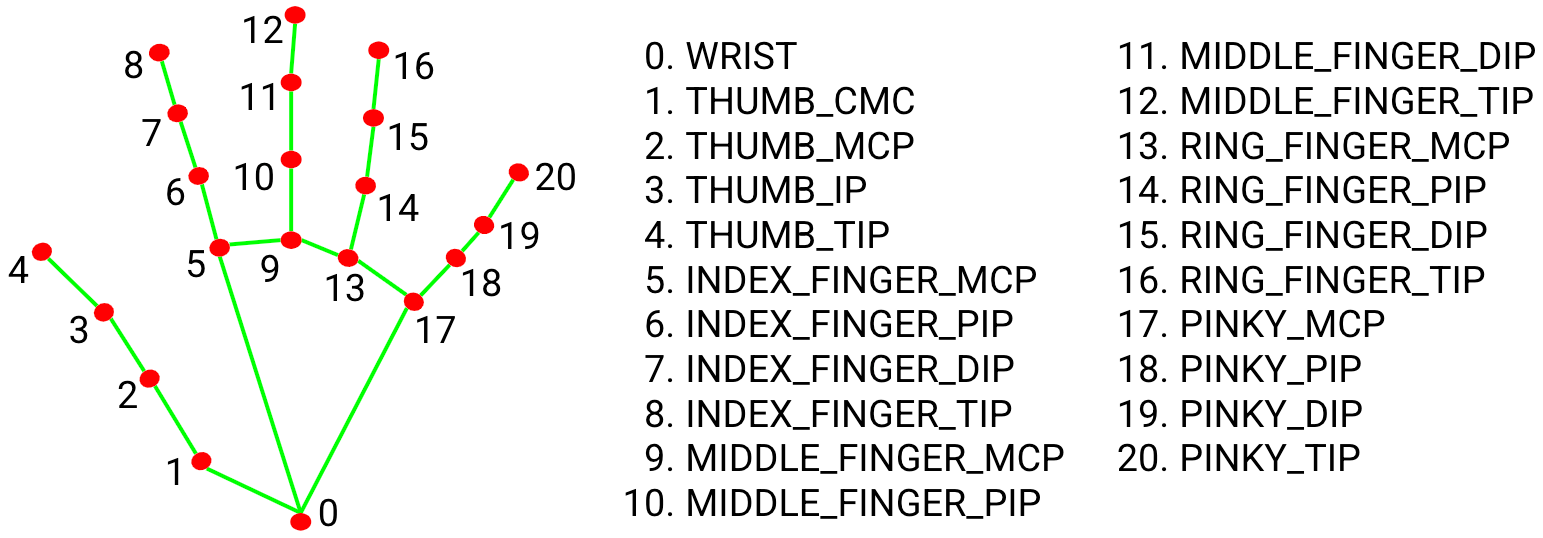
\includegraphics[width=0.6\linewidth]{01_MediaPipe/hand_landmarks.png}
    \end{center}
\end{frame}


% Diapositiva 4: Flujo de funcionamiento
\begin{frame}{Flujo de funcionamiento}
    \begin{enumerate}
        \item Captura de datos desde una cámara o archivo.
        \item Procesamiento mediante el gráfico de MediaPipe.
        \item Obtención de resultados como coordenadas de puntos clave o segmentación.
    \end{enumerate}
    \begin{center}
        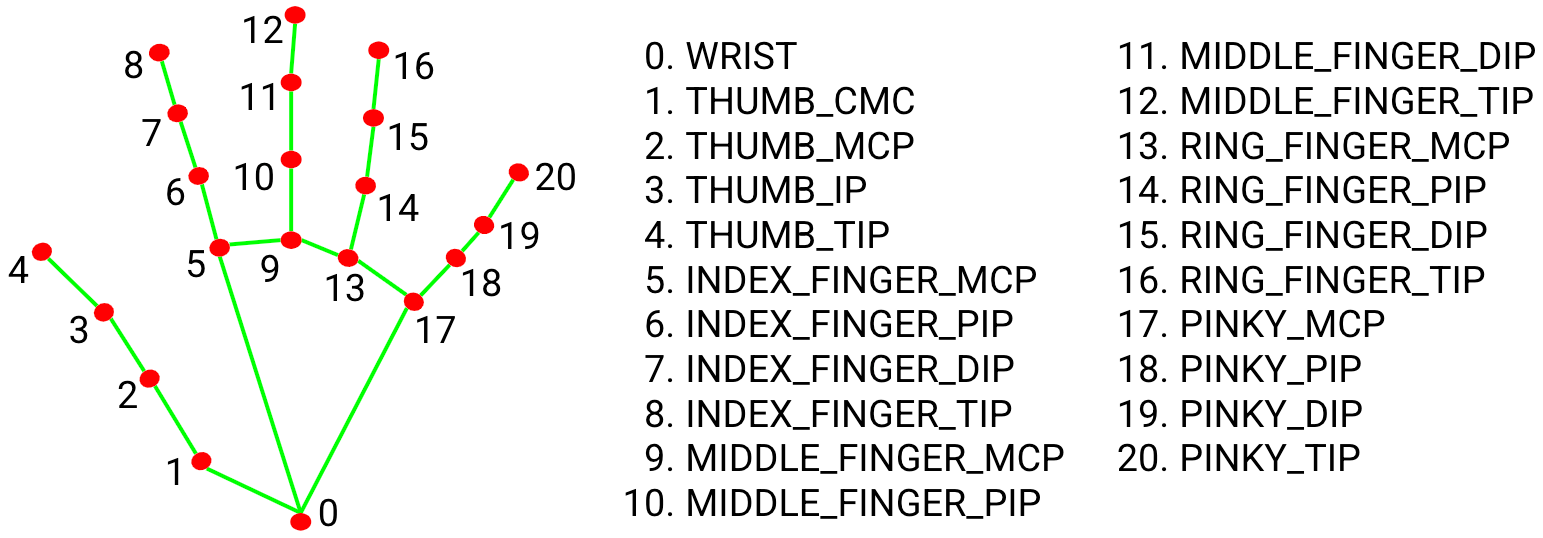
\includegraphics[width=0.6\linewidth]{01_MediaPipe/hand_landmarks.png}
        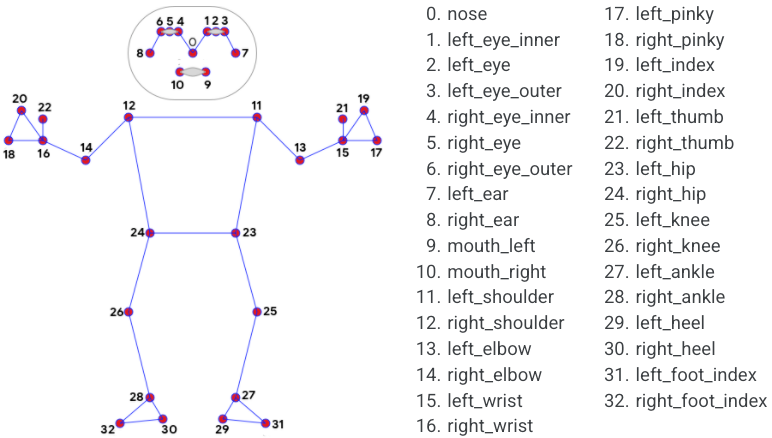
\includegraphics[width=0.6\linewidth]{01_MediaPipe/pose_landmarks.png}
    \end{center}
\end{frame}

